\documentclass[11pt, a4paper]{article}
\usepackage{cmap}
\usepackage{graphicx}
\usepackage[T2A]{fontenc}
\usepackage[utf8]{inputenc}
\usepackage[russian]{babel}
\usepackage{amsmath, amssymb}
\usepackage[usenames]{color}
\usepackage{colortbl}
\usepackage{fancyhdr}
\usepackage{enumitem}
\usepackage{titlesec}
\usepackage{multicol}
\usepackage{tabularx}
\usepackage{caption}
\usepackage{tikz}
\usetikzlibrary{positioning, arrows.meta}
\usepackage[backend=biber, style=numeric, sorting=none]{biblatex}
\DefineBibliographyExtras{russian}{\protected\def\bibrangedash{\textendash\penalty\hyphenpenalty}}
\AtBeginBibliography{\sloppy}
\renewcommand*{\bibfont}{\small}
\addbibresource{source.bib}
\usepackage{csquotes}
\usepackage[hidelinks]{hyperref}
\usepackage{xurl}
\usepackage{placeins}

\usepackage{geometry}
\geometry{
  a4paper,
  top=30mm,
  right=5mm,
  bottom=20mm,
  left=5mm,
  headheight=61pt
}
\setlength{\columnsep}{8mm}
\raggedcolumns  % не растягивать колонки по высоте
\emergencystretch=2em
\renewcommand{\topfraction}{0.95}
\renewcommand{\bottomfraction}{0.6}
\renewcommand{\textfraction}{0.05}
\renewcommand{\floatpagefraction}{0.85}
\setcounter{topnumber}{3}\setcounter{totalnumber}{4}

\newcommand{\mydate}{Ноябрь, 2026}
\newcommand{\myauthor}{В. Алексеев, С. Зинина, И. Коновалов, В. Горбатенко, А. Соколова}

\fancyhf{}
\fancyhead[L]{\large \textit{Научная студия 2026. Вычислительная онкология. Классификация.}}
\fancyfoot[C]{\thepage}
\pagestyle{fancy}

\fancypagestyle{firstpage}{
  \fancyhf{}
  \fancyhead[L]{\hspace{-15pt}
\includegraphics[width=0.3\linewidth]{fig/cu_logo.png}}
  \fancyhead[R]{\mydate\\\textit{\myauthor}\\}
  \fancyfoot[C]{\thepage}
}

\newcommand{\code}[1]{\texttt{\small #1}}

\begin{document}
\thispagestyle{firstpage}
\begin{multicols}{2}
\section*{Материалы и методы}
\subsection*{Модели машинного обучения}
Для прогнозирования локального рецидива рака ротоглотки по клиническим и КТ-радиомическим признакам обучены логистическая регрессия, дерево решений и случайный лес в библиотеке scikit-learn версии 1.9.1~\cite{Pedregosa2011}. Логистическая регрессия выбрана как линейная модель с регуляризацией: при малом числе рецидивов ограничение величины коэффициентов снижает риск подгонки к отдельным пациентам. Использован квадратичный штраф с обратной силой регуляризации 0,1. Дерево решений позволяет учесть пороговые зависимости и взаимодействия клинических и радиомических характеристик. Для ограничения сложности максимальная глубина дерева ограничена значением 3, а лист содержал не менее 8 обучающих пациентов. Случайный лес из 300 деревьев выбран как ансамбль, усредняющий нестабильные решения отдельных деревьев~\cite{Breiman2001}. Глубина его деревьев также ограничена значением 3, минимальное число пациентов в листе составляет 5; при поиске разбиения рассматривается случайный набор признаков размером с квадратный корень из их числа. Из-за редкости рецидива во всех моделях использованы веса классов, обратно пропорциональные их частотам; для леса они рассчитаны отдельно в каждой бутстреп-выборке. Настройки заданы до сравнения на валидации и по её результатам не менялись.

\subsection*{Обучение и сравнение моделей}
Использована аналитическая таблица недели 4: 140 пациентов, 12 с рецидивом, 31 исходный признак. Сохранены идентификаторы тестовой выборки недели 5: 35 пациентов, из них 3 с исходом~1. Из оставшихся 105 пациентов стратифицированным по исходу случайным разделением выделена валидационная выборка объёмом 20\%: 21 пациент, 2 с рецидивом. Обучающая выборка содержит 84 пациента, 7 с рецидивом. Стратификация сохраняет представительство редкого исхода, а небольшая валидационная доля оставляет больше событий для обучения~\cite{Riley2020}. Для разделения и стохастических моделей зафиксировано начальное значение генератора 42; состав выборок проверен на отсутствие пересечений.\vspace{6pt}\\
Подготовка признаков включена в каждую модель и заново настроена только по 84 обучающим пациентам: готовые преобразованные таблицы недели 5 не использованы, поскольку их параметры рассчитаны также по будущей валидационной выборке. Пропуски 20 количественных и 4 порядковых признаков заполнены обучающими медианами, устойчивыми к асимметрии; значения стандартизованы обучающими средними и стандартными отклонениями для сопоставимого штрафа в регрессии. Количественные признаки не логарифмировались: для этого сравнения сохранена единая простая подготовка без дополнительного подбора преобразований при семи событиях. Порядковые коды сохраняют порядок категорий, три бинарных признака представлены нулями и единицами. Пропуски категориальных признаков заполнены обучающими модами. Четыре номинальных признака закодированы индикаторами с исключением одной опорной категории; категории с частотой менее 5 объединены для уменьшения числа неустойчивых оценок. Неизвестные категории валидации отнесены к редкой группе, если она сформирована, иначе представлены нулями. Добавлен индикатор пропуска степени дифференцировки, так как отсутствие оценки может характеризовать доступность биопсийного материала. Получено 36 числовых признаков; параметры без пересчёта применены к валидации.\vspace{6pt}\\
Основная мера сравнения~--- доля верных ответов на валидационной выборке; та же мера на обучении приведена для оценки подгонки. Из-за дисбаланса дополнительно рассчитаны чувствительность, средняя полнота двух классов и матрицы ошибок, а ориентиром служит постоянный прогноз отсутствия рецидива. При двух событиях валидации оценки неустойчивы, поэтому высокая доля верных ответов сама по себе не подтверждает способность выявлять рецидив. Тестовая выборка не использована для настройки подготовки, обучения, предсказаний и сравнения моделей; она отложена для однократной итоговой оценки после фиксации модели.
\subsection*{Ссылки}
\printbibliography[heading=none]
\end{multicols}

\clearpage
\section*{Приложение. Иллюстрации к анализу}

\begin{figure}[!ht]
  \centering
  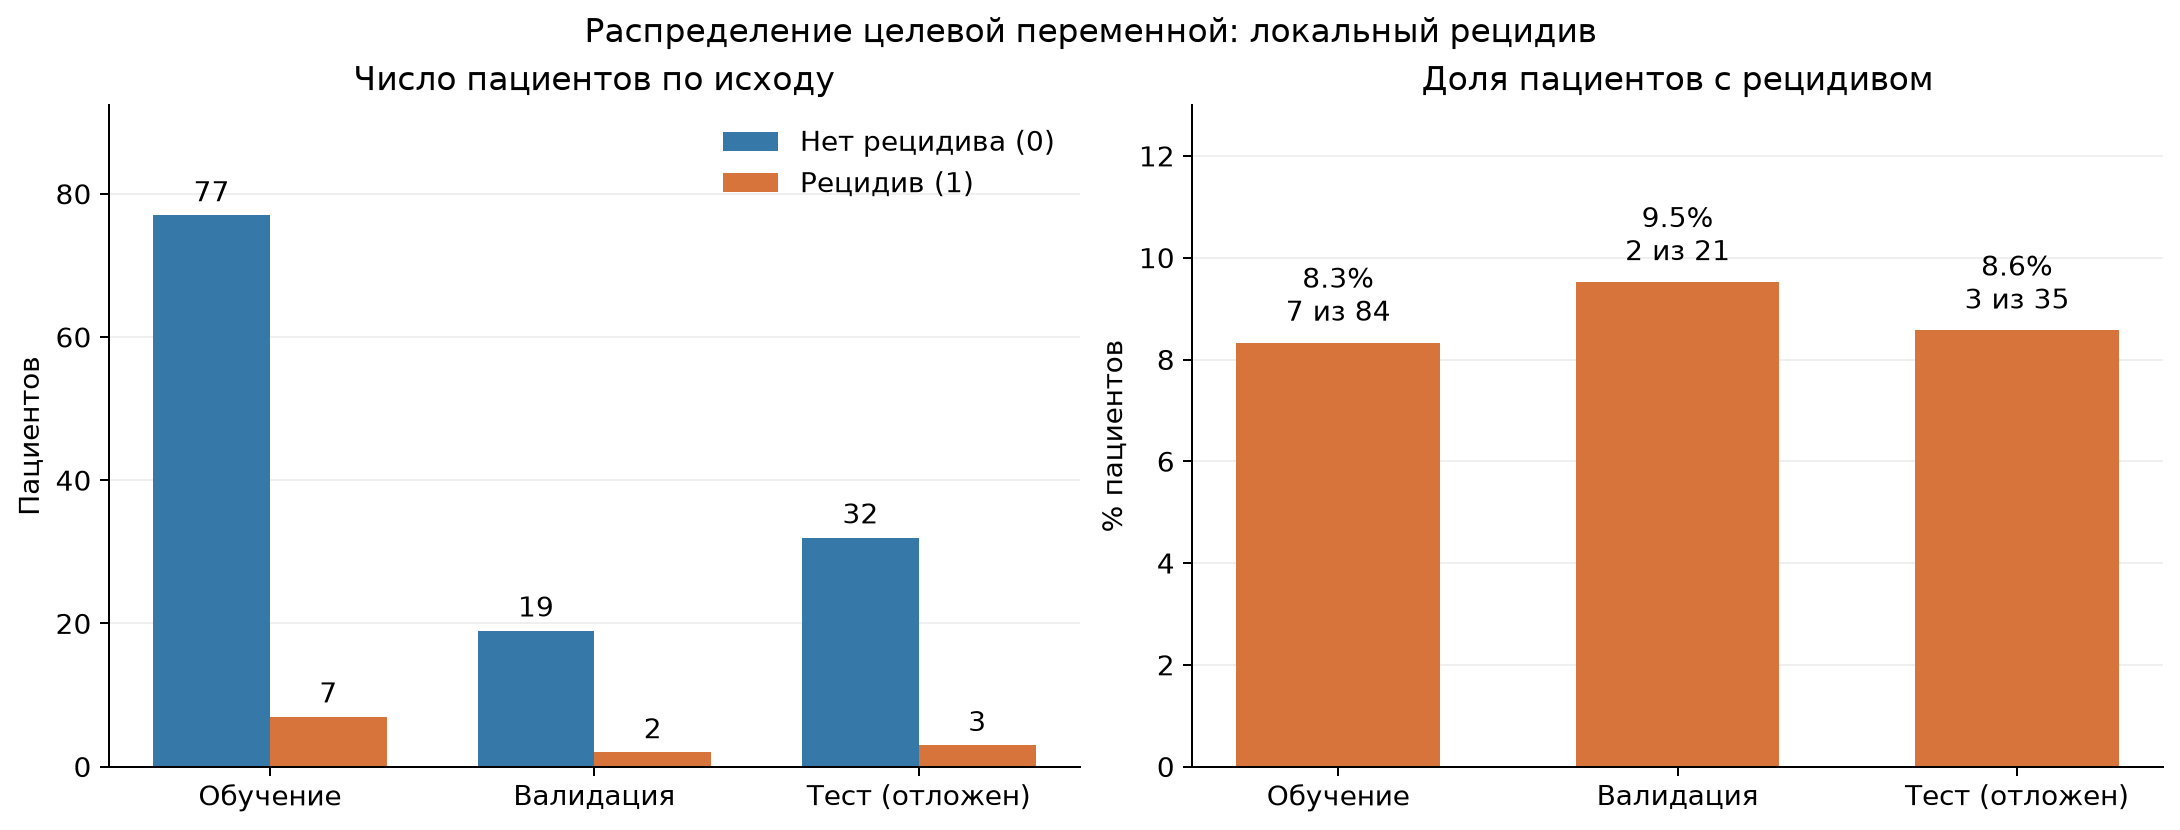
\includegraphics[width=0.92\linewidth]{fig/target_distribution.png}
  \caption{Распределение локального рецидива по выборкам: число пациентов с каждым исходом и доля пациентов с рецидивом. Тестовая выборка показана только для описания её состава.}
  \label{fig:target-distribution}
\end{figure}

\begin{figure}[!ht]
  \centering
  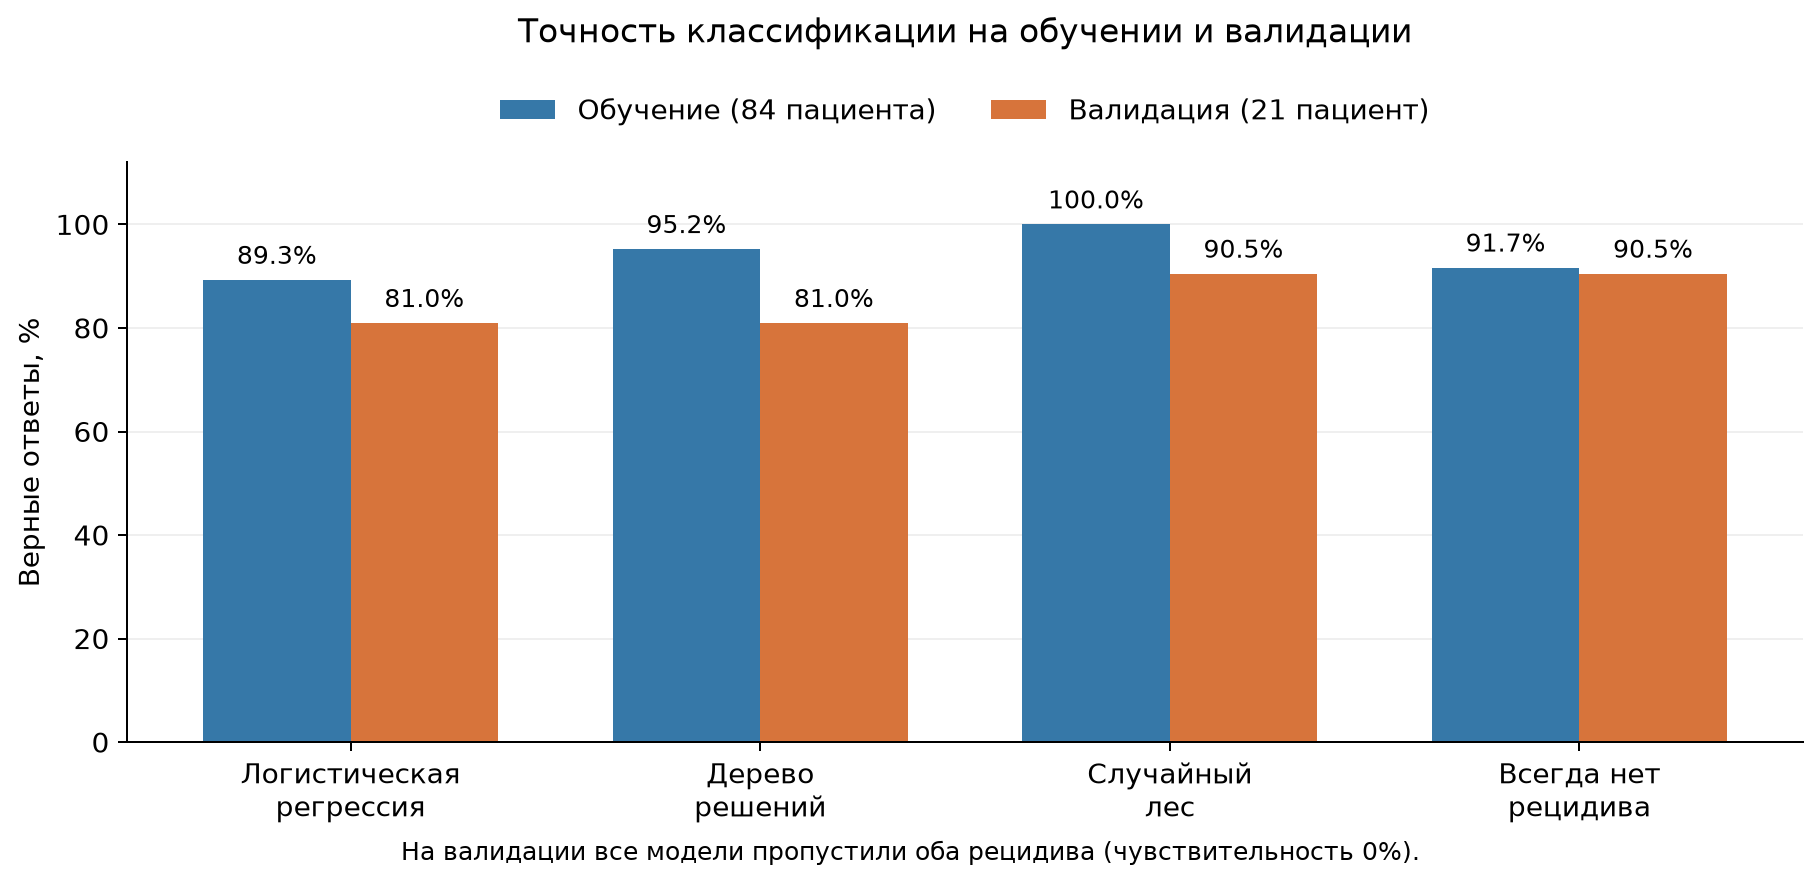
\includegraphics[width=0.92\linewidth]{fig/model_accuracy.png}
  \caption{Доля верных ответов на обучающей и валидационной выборках для трёх моделей и постоянного прогноза отсутствия рецидива. Точность случайного леса на валидации совпадает с постоянным прогнозом; все модели пропустили оба рецидива.}
  \label{fig:model-accuracy}
\end{figure}

\clearpage
\section*{Матрицы ошибок}

\begin{figure}[!ht]
  \centering
  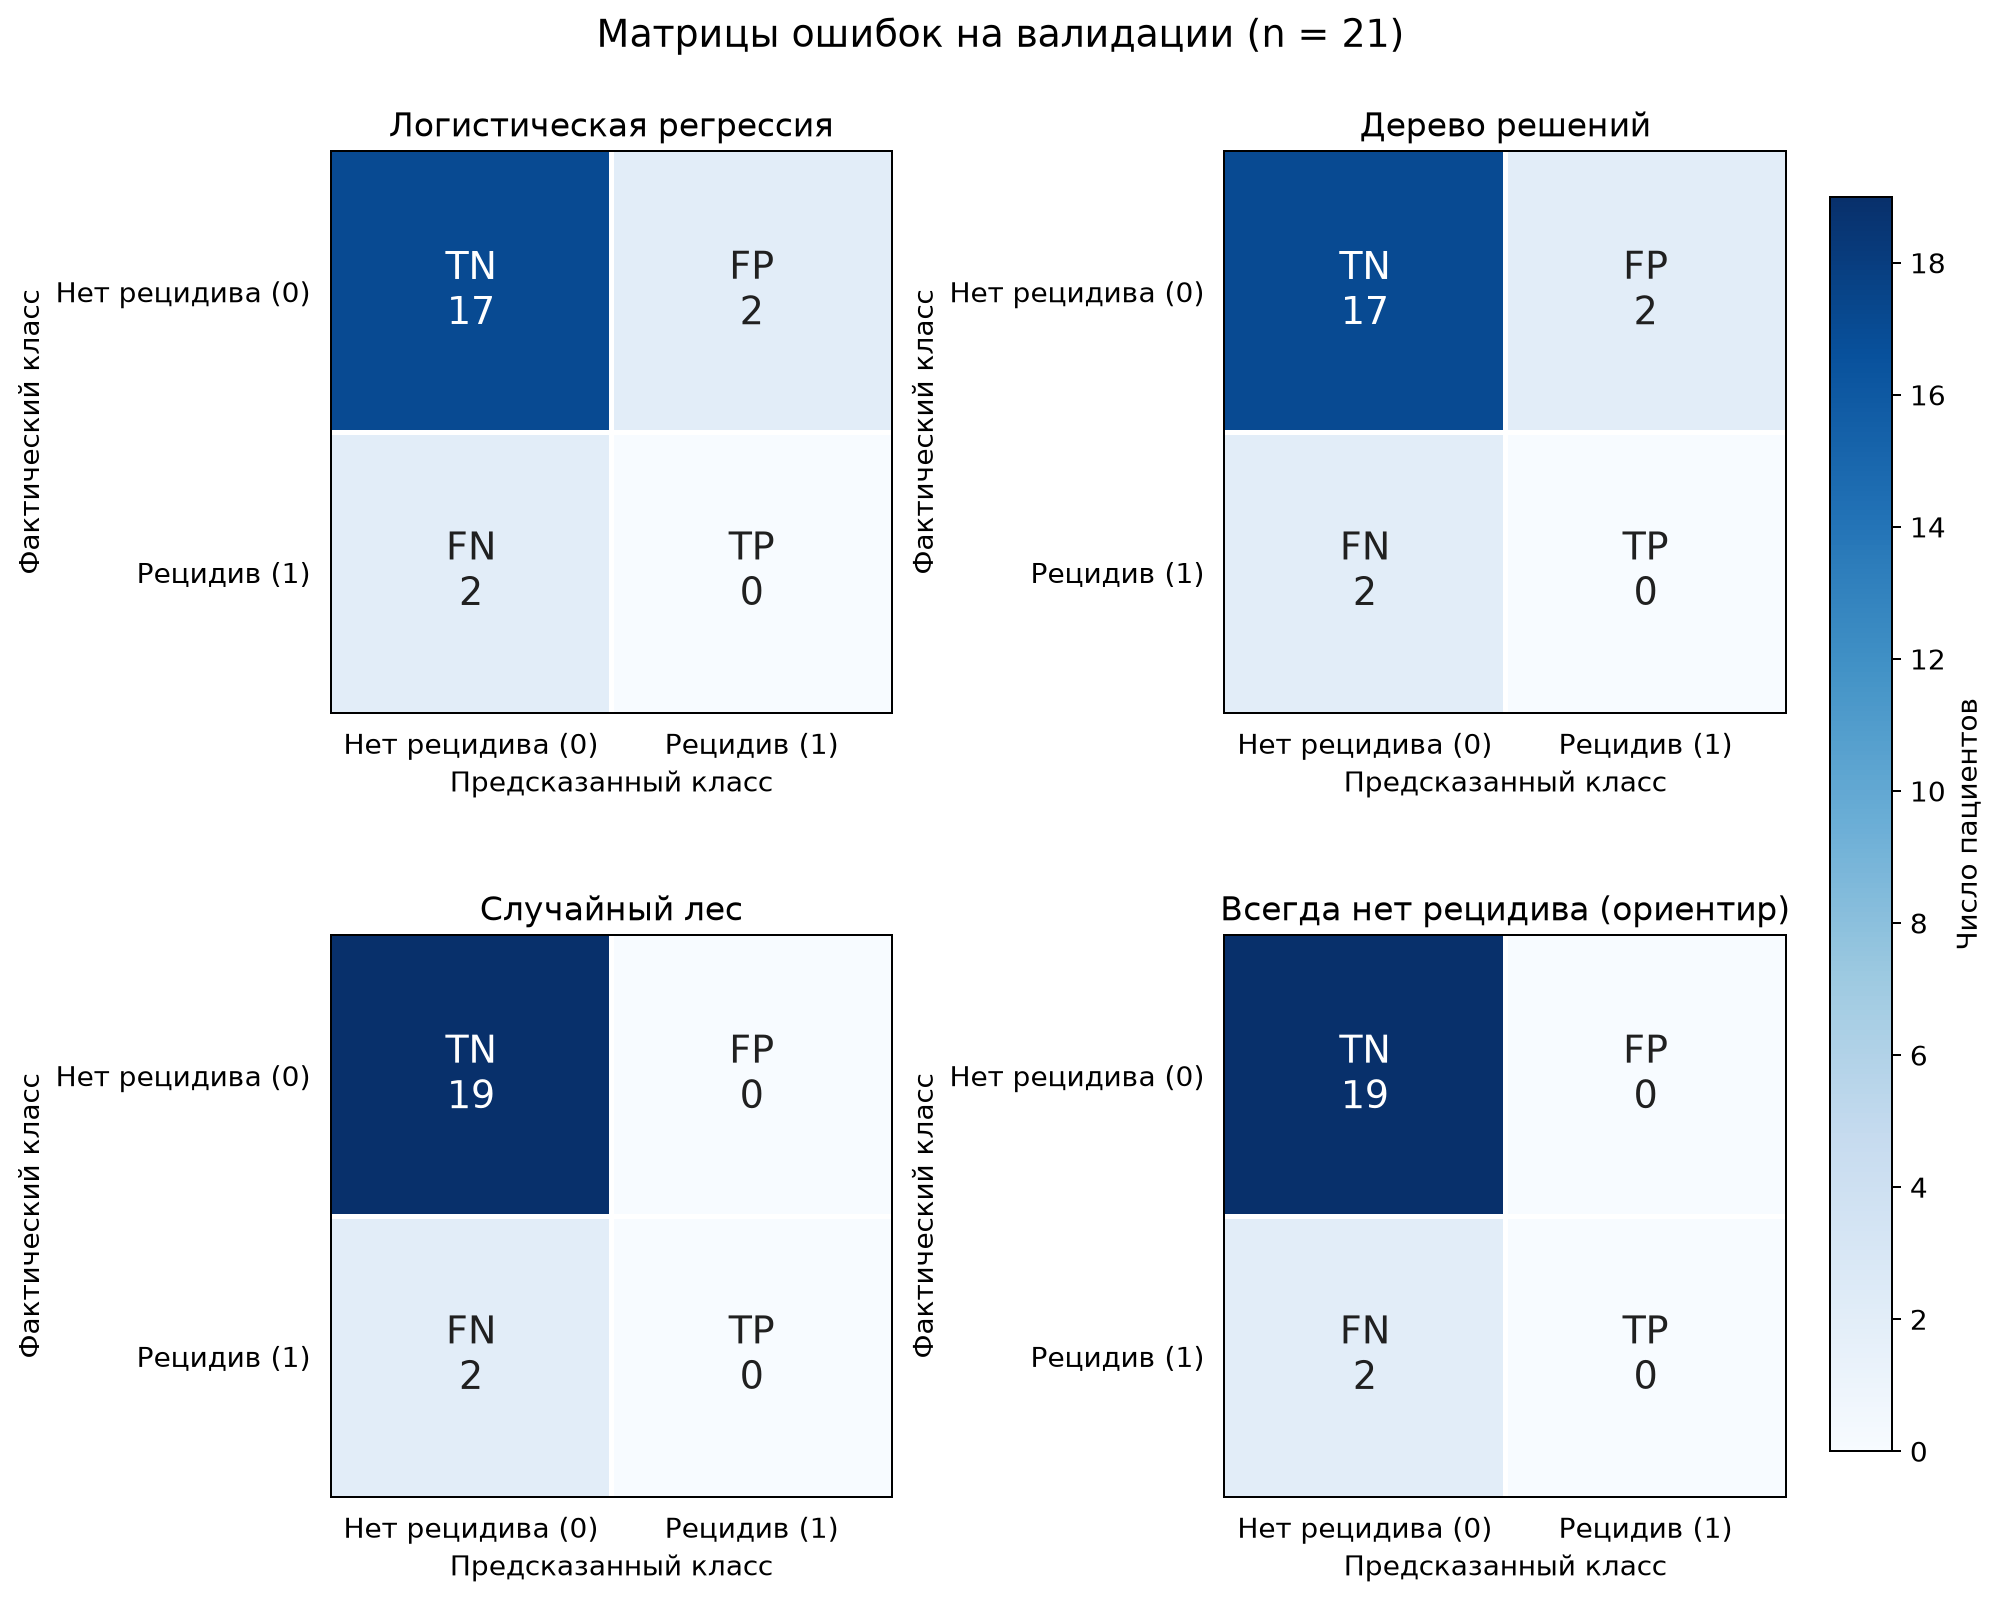
\includegraphics[width=0.92\linewidth]{fig/confusion_matrices.png}
  \caption{Матрицы ошибок на валидационной выборке из 21 пациента. Строки соответствуют фактическому классу, столбцы~--- предсказанному. В ячейках приведены число пациентов и обозначения истинно отрицательных (TN), ложноположительных (FP), ложноотрицательных (FN) и истинно положительных (TP) результатов. Для всех четырёх матриц используется общая цветовая шкала.}
  \label{fig:confusion-matrices}
\end{figure}

\end{document}
